\section{Validation des Fonctions}
Pour effectuer la validation de notre système nous avons téléversé notre projet sur le FPGA, la partie Hardware grâce au SOPC et la partie logicielle à l'aide de l'environnement Eclipse qui nous a permit de lancer/tester et débugger notre projet directement sur la maquette d'évaluation.

\begin{figure}[h]
    \begin{center}
      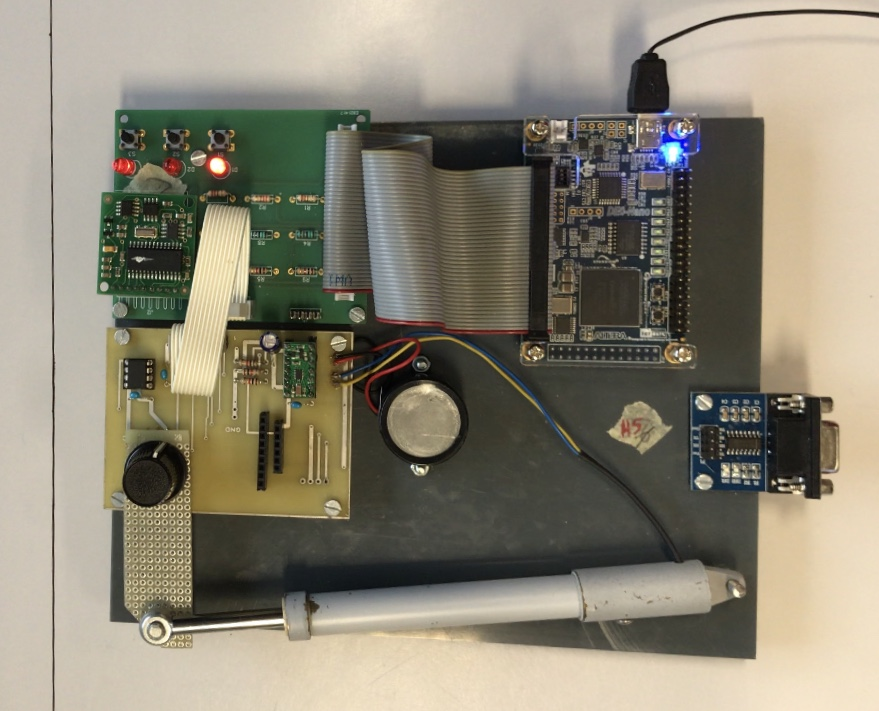
\includegraphics[width=0.7\textwidth]{images/maquette.jpg}
      \caption{Maquette validation projet}
    \end{center}
  \end{figure}

  Nous avons réalisé trois tests pour tester le bon fonctionnement du projet. Pour le premier test nous avons utilisé un GBF qui nous a permit d'injecter directement sur le GPIO, du FPGA attribué, une fréquence qu'on peut modifier pour venir simuler la sortie de l'anémomètre. Après observation la fréquence est bien actualisée toutes les secondes comme demandé dans le cahier des charges. Pour le second test nous venons tester la fonction gestion vérin avec la fonction interface Homme système les boutons nous on permit de tester le bon fonctionnement qui contrôle le signal PWM du vérin. Pour la dernière fonction qui est l'asservissement du système complet nous observons un maintient du cap définit dans le logicielle téléversé sur la maquette de développement et que celle-ci respecte bien le cap fixé avant chaque passage en mode automatique.